\chapter{EVIDENCE OF MICROBURSTS OBSERVED NEAR THE EQUATORIAL PLANE IN THE OUTER VAN ALLEN RADIATION BELT}\label{CH:mageis_microburst}

\section{Contribution of Authors and Co-Authors} 
\noindent Manuscript in Chapter 1 \\ 

\noindent Author: Mykhaylo Shumko
\begin{singlespace} \noindent Contributions: Found the microburst event and applied the quasi-linear diffusion theory to the observation. \end{singlespace}
\noindent Co-Author:  Drew L. Turner 
\begin{singlespace} \noindent Contributions: Mentor who helped organize this paper and provided networking opportunities with the Van Allen Probes team. \end{singlespace}
\noindent Co-Author: T. P. O'Brien
\begin{singlespace} \noindent Contributions: Mentor who proposed the quasi-linear diffusion theory analysis and helped with the analysis. \end{singlespace}
\noindent Co-Author:  Seth G. Claudepierre
\begin{singlespace} \noindent Contributions: Visualized the MagEIS data in a way that led to this discovery. Helped process the MagEIS data. \end{singlespace}
\noindent Co-Author: John Sample
\begin{singlespace} \noindent Contributions: Provided analysis advice. \end{singlespace}
\noindent Co-Author: D. P. Hartley
\begin{singlespace} \noindent Contributions: Processed the EMFISIS high resolution data. \end{singlespace}
\noindent Co-Author: Joseph Fennell
\begin{singlespace} \noindent Contributions: Provided advice to interpret the observations.\end{singlespace}
\noindent Co-Author: J. Bernard Blake
\begin{singlespace} \noindent Contributions: Provided advice to interpret the observations and principal investigator of MagEIS. \end{singlespace}
\newpage
\noindent Co-Author: Matina Gkioulidou
\begin{singlespace} \noindent Contributions: Helped correctly use the RBSPICE data. \end{singlespace}
\noindent Co-Author: Donald G. Mitchell
\begin{singlespace} \noindent Contributions: Helped correctly use the RBSPICE data and principal investigator of RBSPICE. \end{singlespace}

\newpage

\section{Manuscript Information}

\begin{singlespace} \noindent Mykhaylo Shumko, Drew L. Turner, T. P. O'Brien, Seth G. Claudepierre, John Sample, D. P. Hartley, Joseph Fennell, J. Bernard Blake, Matina Gkioulidou, and Donald G. Mitchell \end{singlespace}

\begin{singlespace}
\noindent Status of Manuscript: \\
\_\_\_ Prepared for submission to a peer-reviewed journal \\
\_\_\_ Officially submitted to a peer-reviewed journal \\
\_\_\_ Accepted by a peer-reviewed journal \\ 
\_X\_ Published in a peer-reviewed journal
\end{singlespace}

\begin{singlespace}
\noindent Geophysical Research Letters Volume 45, Issue 16 \\
\noindent DOI: 10.1029/2018GL078451
\end{singlespace} 

\newpage

\section{Key Points}
\begin{itemize}
\item First report of direct observation of microbursts at high altitude, near the equatorial plane.
\item Microbursts' duration, flux enhancement, and energy spectra are similar to prior observations in LEO.
\item Microburst generation is not consistent with a single quasi-linear gyroresonant interaction with chorus waves.
\end{itemize}

\section{Abstract}
We present the first evidence of electron microbursts observed near the equatorial plane in Earth's outer radiation belt. We observed the microbursts on March 31st, 2017 with the Magnetic Electron Ion Spectrometer and RBSP Ion Composition Experiment on the Van Allen Probes. Microburst electrons with kinetic energies of 29-92 keV were scattered over a substantial range of pitch angles, and over time intervals of 150-500 ms. Furthermore, the microbursts arrived without dispersion in energy, indicating that they were recently scattered near the spacecraft. We have applied the relativistic theory of wave-particle resonant diffusion to the calculated phase space density, revealing that the observed transport of microburst electrons is not consistent with the hypothesized quasi-linear approximation.

%% ------------------------------------------------------------------------ %%
%
%  TEXT
%
%% ------------------------------------------------------------------------ %%
\section{Introduction}\label{Intro} %%%%%%%%%%%%%%%%%%%%%%%%%%%%%%%%%%%%%%%%%%%%
Since the Van Allen radiation belts were discovered by \citet{Allen1959} and \citet{Vernov1960}, decades of work has focused on understanding their origins and effects on the near-Earth space environment and ionosphere-thermosphere system. The energy content of the outer belt is dominated by energetic electrons, with dynamics controlled by a complex interplay between various source and loss mechanisms. One important loss and acceleration mechanism is gyroresonant diffusion in energy and pitch angle (PA) due to scattering of electrons by plasma waves \citep[e.g.][]{Thorne1980, Walker1993, Summers1998, Meredith2002, Horne2003, Thorne2005, Millan2007, Bortnik2008}.

Chorus waves are commonly associated with PA and energy diffusion. These waves are typically generated by substorm injections into the inner magnetosphere, which lead to a temperature anisotropy of the source electrons with energies up to tens of keV \citep[e.g.][]{Horne2003b, Li2009b}. Since these source electrons drift eastward, chorus is most frequently observed in the dawn sector, but it has been observed at all magnetic local times (MLT) \citep{Li2009}. Chorus waves are believed to generate electron microburst precipitation through wave-particle interactions.

Microbursts are typically defined as an increase of electron flux in or near the atmospheric loss cone that last $< 1$ s \citep[e.g.][]{Anderson1964, Blake1996, Lorentzen2001a}. Empirical and theoretical analyses indicate that microbursts are an important loss process since they can substantially deplete the radiation belt electrons on the order of one day \citep[e.g.][]{Lorentzen2001b, O'Brien2004, Thorne2005, Breneman2017}. Previously, microbursts have been observed in the upper atmosphere in the form of bremsstrahlung X-rays \citep[e.g.][]{Parks1967, Woodger2015, Anderson2017} and directly in low Earth orbit (LEO) \citep[e.g.][]{Nakamura1995, Nakamura2000, Blake1996, Lorentzen2001a, Lorentzen2001b, O'Brien2003, O'Brien2004, Lee2005, Lee2012, Blum2015, Crew2016, Breneman2017, Mozer2018}.
 
We observed for the first time, microburst-like signatures near their hypothesized origin within the heart of the outer radiation belt. The unique microburst observations we report here were possible with the Van Allen Probe-A's (RBSP-A) Magnetic Electron Ion Spectrometer's (MagEIS) fast sampling rate (${\sim} 11$ ms), and RBSP Ion Composition Experiment's (RBSPICE) PA coverage. The observed microbursts' duration, energy spectra, and energy dispersion signature were similar to microbursts previously reported from LEO. Furthermore, we simultaneously observed structureless ``hiss-like'' whistler mode wave power in the lower band chorus frequency range \citep{Li2012}. From previous observations in LEO \citep[e.g.][]{Blake1996}, it is believed that microbursts result from the impulsive scattering of electrons into or near the loss cone, which is on the order of a few tens of degrees in LEO. With this assumption, high altitude microburst observations near the magnetic equator should be very difficult to make since the atmospheric loss cone there is only a few degrees wide. Thus, the loss cone is smaller than the angular resolution of most particle detectors. Even when an instrument is observing the loss cone, the instrument's field of view will include some portion of the trapped population. The trapped electron flux is typically orders of magnitude higher than that in the loss cone, so that microbursts scattered into the loss cone will be obscured. We present observational evidence that suggests that the sudden impulse of electrons studied here is consistent with the creation of microbursts. Furthermore, these microbursts were scattered over a broad PA range outside of the loss cone, though the loss cone was not directly observed by MagEIS and RBSICE.

This paper explores the properties of the observed microbursts by utilizing in-situ RBSP measurements of waves and particles. This unique high altitude point of view enables us to test whether the observed microburst scattering is consistent with a quasi-linear diffusion process. We have tested this hypothesis with in-situ electron phase space density (PSD) measurements and the relativistic theory of wave-particle resonant diffusion \citep{Walker1993, Summers1998} to determine if the microburst electrons diffused in PA and energy.

\section{Spacecraft Instrumentation} \label{sc} %%%%%%%%%%%%%%%%%%%%%%%%%%%%%%%%%%%%%%%%%%%%
NASA's RBSP mission \citep{Mauk2013}, launched on August 30th, 2012, consists of a pair of identically instrumented spacecraft. Their orbit and instrumentation are uniquely configured to enrich our understanding of the particles and waves in the inner magnetosphere. The RBSP spacecraft are in highly elliptical, low-inclination orbit, with perigee of ${\sim}600$ km and apogee of ${\sim}30,000$ km altitude. Their attitude is maintained by spin-stabilization with a period of ${\sim}11$ s and the spin axis is roughly sun-pointing. In this analysis, energetic electron measurements from MagEIS \citep{Blake2013} and RBSPICE \citep{Mitchell2013} were used, complemented by magnetic field and wave measurements from Electric and Magnetic Field Instrument and Integrated Science (EMFISIS) \citep{Kletzing2013}.

We observed these microbursts with RBSP-A's MagEIS low energy instrument (MagEIS-A) which measures 20-240 keV electrons. It has an angular acceptance of $3^\circ - 10^\circ$ in the spacecraft spin plane, and $20^\circ$ perpendicular to the spin plane. MagEIS-A has a high rate data mode which samples at 1000 angular sectors per spacecraft spin (11 ms cadence). MagEIS low on RBSP-B on the other hand samples at 64 angular sectors per spacecraft spin (172 ms cadence), so it was only used for context.

To expand the PA coverage of MagEIS-A, we used the RBSPICE-A time-of-flight instrument. RBSPICE-A measures electron energies in the range of 19 keV - 1 MeV with a fan of six telescopes (the sixth telescope is used only for calibration and was excluded from this analysis). These telescopes have an overall acceptance angle of $160^\circ$ by $12^\circ$ which allows them to simultaneously sample a substantial part of the Pitch Angle Distribution (PAD). RBSPICE-A gathers data over 32 sectors per spacecraft spin ($\approx 310$ ms cadence) and each sector is divided into three sub-sectors corresponding to three measurement modes \citep{Manweiler2018}. At the time of the observation, the sub-sector used for electron measurements had an accumulation time of $77$ ms. We used RBSPICE-A's Electron Basic Rate (EBR) telemetry data in this analysis which is not averaged, though it is an integral energy channel.

To understand the dynamics of the local magnetic field, we used the EMFISIS instrument. EMFISIS provides measurements of the DC magnetic field with flux gate magnetometers. In addition, it measures electromagnetic waves from 10 Hz to 500 kHz with search coil magnetometers. The spectral matrix and burst data products used in this analysis were from the EMFISIS waveform receiver (WFR) (10 Hz - 12 kHz) and the high frequency receiver (10 kHz - 500 kHz). Burst data were selectively captured at a 35 kHz sample rate, and the survey mode spectral matrix data was captured every 6s.

\section{Observations} \label{obs}
MagEIS-A and RBSPICE-A observed the microburst-like signatures on March 31st, 2017 at $\mathrm{L}^* \approx 6$ and $\mathrm{MLT} \approx 19$, calculated with the Tsyganenko 2004 magnetic field model \citep{Tsyganenko2005}. The magnetosphere was in the recovery phase of a storm, with minimum Dst of -75 nT observed on March 27th. The local electron number density was on the order of $1 \ \mathrm{cm}^{-3}$ at this time, so both RBSP spacecraft were located outside the plasmasphere. The two spacecraft were separated by 1700 km, at magnetic latitudes $\lambda {\approx} -19^\circ$ and $\lambda {\approx} -18^\circ$ for RBSP-A and RBSP-B, respectively.

MagEIS-A observed microburst electron flux $(J)$ at energies < 92 keV around 11:17 UT as shown in panel (a) in Fig. \ref{fig1}. For directional information, panel (b) in Fig. \ref{fig1} shows flux as a function of local pitch angle ($\alpha_{L}$) and time for 46-66 keV electrons. Electrons that traveled towards the northern hemisphere had $\alpha_{L} < 90^\circ$ and southern hemisphere had $\alpha_{L} > 90^\circ$. The interval between the two vertical dashed black lines contain the four microbursts examined in this study. We observed these microbursts at $\alpha_{L} < 50^\circ$, but MagEIS-A did not sample into the $0^\circ$ loss cone.

Figure \ref{fig1} panel (c) shows the EMFISIS WFR data from RBSP-A. Between 11:17:05 and 11:17:10 UT, we observed an isolated burst of whistler mode wave power in the frequency range $0.1 < \omega < 0.3 \ \Omega_{ce0}$, where $\Omega_{ce0}$ is the equatorial electron gyrofrequency. No individual rising or falling tone elements were observed during this period, and the waves appeared more ``hiss-like'' \citep[e.g.][]{Li2012}. This wave was near-parallel propagating (evidence shown in Appendix \ref{appendixa}) and about 10 minutes later, weak chorus rising tone elements were observed (not shown).

Panels (d)-(f) in Fig. \ref{fig1} are in the same format as panels (a)-(c), but for RBSP-B. An injection or boundary was observed with RBSP-B at 11:16:50 UT and RBSP-A observed a similar feature soon after 11:18 UT (not shown).

\begin{figure}
\centering
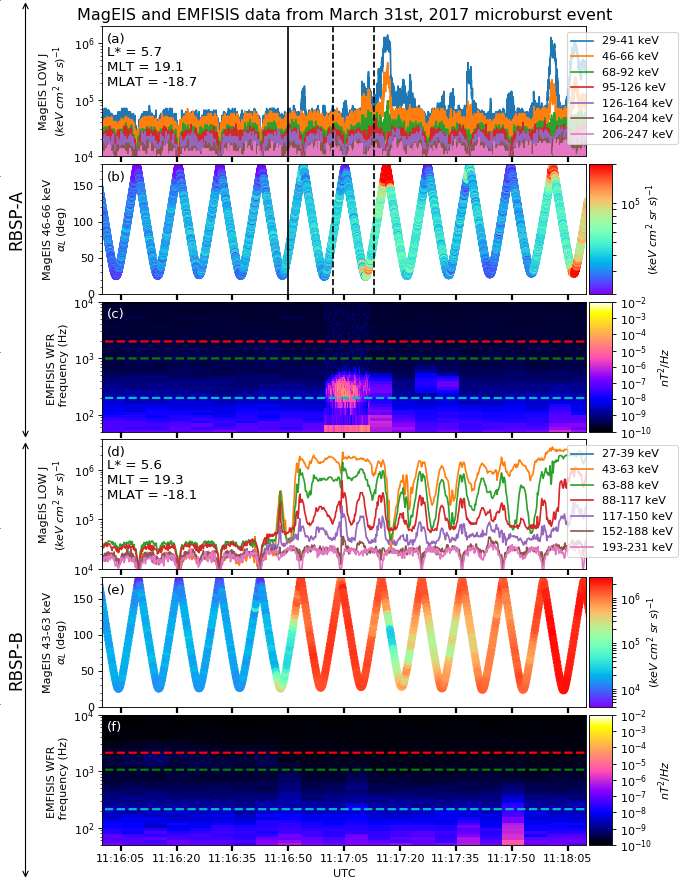
\includegraphics[width=0.75\textwidth]{2_fig1.png}
\caption{Electron and wave conditions from the MagEIS-A and EMFISIS WFR sensors for the microburst time interval. Panels (a), (b), and (c) are from RBSP-A with its position information annotated in panel (a). Panels (d), (e), and (f) are from RBSP-B with its position information annotated in panel (d). Panel (a) is the MagEIS-A high rate timeseries. Panels (b) and (e) show the evolution of the MagEIS-A $J$ as a function of $\alpha_{L}$ from the ${\sim} 40$ to ${\sim} 60$ keV channel. Every 10th point is shown in panel (b). The solid black line in panels (a) and (b) mark the end of the time period used for the PSD fit extrapolation analysis explained in section \ref{analysis}. The dashed black lines in panels (a) and (b) show the time interval used for the observed microburst PSD. Panels (c) and (f) show the EMFISIS WFR spectra, with the available burst data superposed. The red, green, and cyan traces are equatorial $f_{ce0}$, $f_{ce0}/2$, and $f_{ce0}/10$, respectively. }
\label{fig1}
\end{figure}

A zoomed-in version of Fig. \ref{fig1} panels (a) and (b) is shown in Fig. \ref{fig2}. Panel (a) shows the four microburst-like signatures observed between 11:17:10 and 11:17:12 UT, at energies up to 92 keV. The observed duration of the microbursts was 150 - 500 ms, and they did not arrive dispersed in energy, which indicates that they were recently scattered near the spacecraft location. We use IRBEM-Lib, a library dedicated to radiation belt modeling \citep{irbem}, to calculate the mirror point altitudes, which were found to be above LEO. Panel (b) shows the RBSPICE-A EBR time series with the group of microbursts observed at the same time as in panel (a). To understand the timing relationship between the MagEIS-A and RBSPICE-A observations, we marked the times when MagEIS-A observed the four microbursts by vertical black arrows in panels (a) and (b). MagEIS-A observed the first microburst $\sim 0.5$ s before RBSPICE-A. The bounce period of locally mirroring, 100 keV electrons was $\sim 0.8$ s, so this was unlikely to have been a returning bounce. This evidence confirms that these microburst signatures are packets of electrons and not a boundary moving back and forth at RBSP-A's location. To understand the PA extent of these microbursts, panel (c) shows the 29-41 keV MagEIS-A $J$ and RBSPICE-A EBR as a function of $\alpha_{L}$ and time. The microburst $J$ was observed by MagEIS-A between $25^\circ < \alpha_L < 50^\circ$ and RBPICE-A between $100^\circ < \alpha_L < 160^\circ$, with the highest intensities close to $\alpha_L = 90^\circ$. RBSPICE-A observed a 10-80\% enhancement in count rate over those PAs with the evidence presented in Appendix \ref{appendixa}.

\begin{figure}
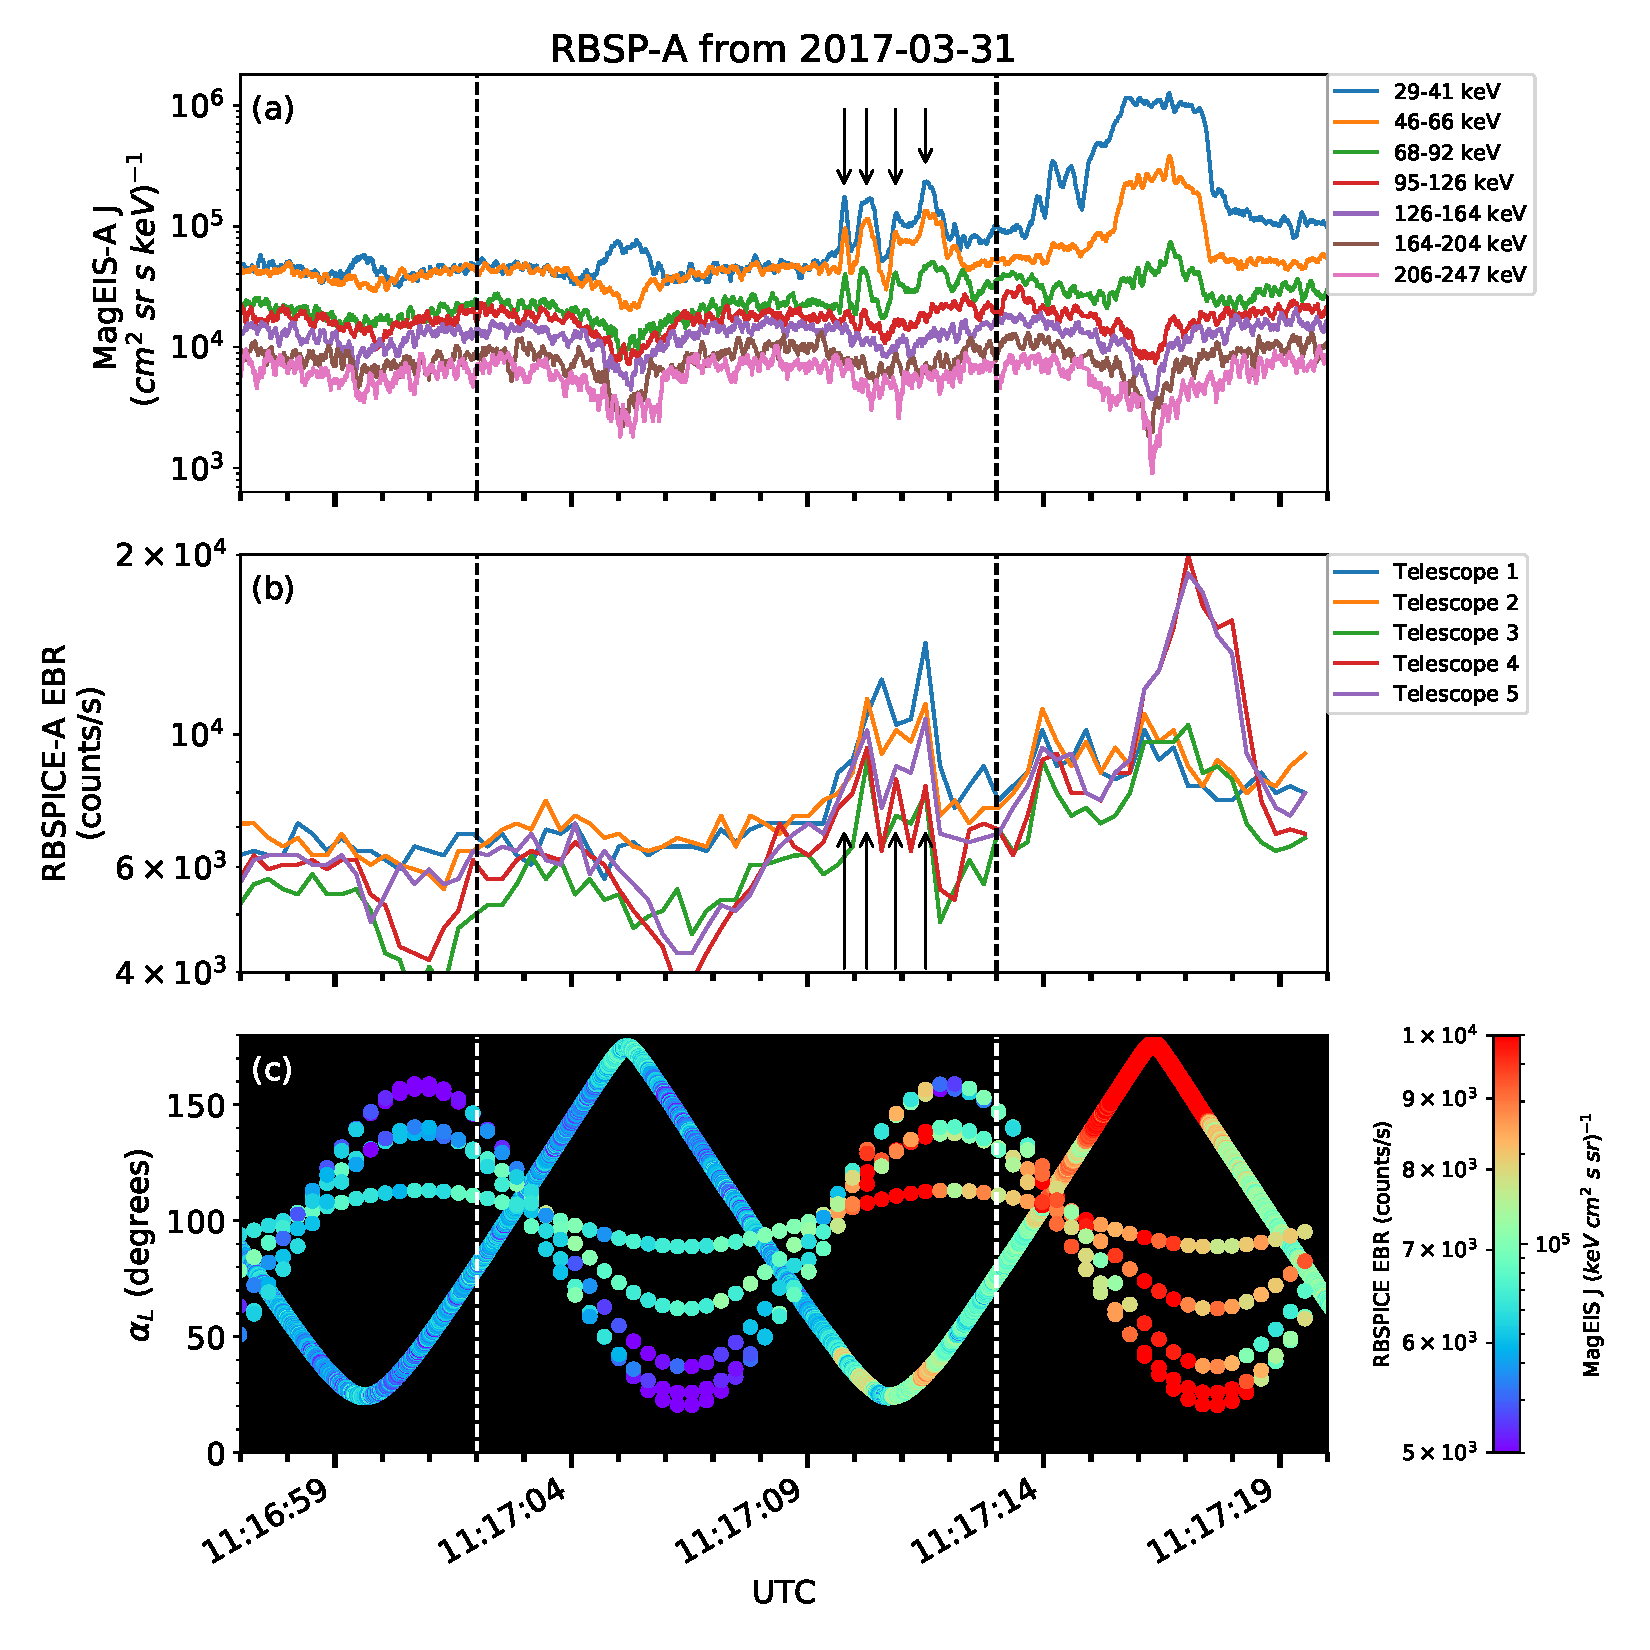
\includegraphics[width=\textwidth]{2_fig2_v2.pdf}
\caption{Panel (a) shows the MagEIS-A high rate timeseries. Panel (b) shows the RBSPICE EBR count rate timeseries for $> 19$ keV electrons. The microbursts were observed between 11:17:10 - 11:17:12 UT and are indicated with the vertical black arrows in panels (a) and (b) for MagEIS-A times. Panel (c) shows the RBSPICE EBR (family of relatively sparse sampled curves) and MagEIS-A $J$ from the 29-41 keV energy channel (single curve) as a function of $\alpha_{L}$. The vertical dashed lines show the time interval for the PSD analysis.}
\label{fig2}
\end{figure}

\section{Analysis} \label{analysis} %%%%%%%%%%%%%%%%%%%%%%%%%%%%%%%%%%%%%%%%%%%%%%%%%%%%%%%%
First, we estimated the microburst energy spectra. For each microburst shown in Fig. \ref{fig2}, its flux was averaged and baseline subtracted using the method from \citet{O'Brien2004} and then fit with an exponential function. The calculated exponential E-folding energy was found to vary between 25 and 35 keV, which is consistent with spectra derived from prior measurements \citep{Datta1997, Lee2005, Lee2012}.

We then tested the hypothesis that the microburst electrons were transported in energy and PA by a single chorus wave. We used a procedure similar to sections 3.1 and 4.5 in \citet{Meredith2002} which we describe below.

\subsection{Microburst and Source PSD} \label{psd_sec}
We estimated the electron PSD, $f(p_\perp, p_{||})$ where $p_\perp$ and $p_{||}$ are the perpendicular and parallel components of the electron momentum relative to the local magnetic field, for the microburst time period. MagEIS-A $J(E, \alpha_{L})$ was averaged between 11:17:02 and 11:17:13 UT and binned by $\alpha_{L}$ into $5^\circ$ bins. Then, we assumed the conservation of the first adiabatic invariant and mapped $\alpha_{L}$ to equatorial PA, $\alpha_{eq}$. The binned $J(E, \alpha_{eq})$ was then converted to $f(p_\perp, p_{||})$ via

\begin{equation}
f(p_\perp, p_{||}) = \frac{J(E, \alpha_{eq})}{p^2},
\label{psd_eq}
\end{equation} where $p = \sqrt{p_\perp^2 + p_{||}^2}$. Lastly, $\alpha_{eq}$ was used to separate $p$ into $p_\perp$ and $p_{||}$ via

\begin{equation}
\frac{p_{||}}{m_e c} = \frac{\sqrt{E(E+2E_0)} \cos{(\alpha_{eq})}}{E_0}
\end{equation} 

\begin{equation}
\frac{p_{\perp}}{m_e c} = \frac{\sqrt{E(E+2E_0)} \sin{(\alpha_{eq})}}{E_0}
\end{equation} where $c$ is the speed of light, $E$ is the kinetic energy, $m_e$ is the electron mass, and $E_0$ is the electron rest energy. The observed $f(p_\perp, p_{||})$ in dimensionless momentum space is shown in Fig. \ref{fig3} in all panels between the $p_{||}$ axis and the white dotted lines. The bright spot in $f(p_\perp, p_{||})$ in the upper $p_{||}$ plane represents the four microbursts.  Along with the observed PSD, we use Fig. \ref{fig3} to explore the various PSD extrapolation and diffusion model assumptions which are described below.

We proceed under the assumption that the source of the microburst electrons is not likely to be at the latitude of the observation, and is closer to the magnetic equator. To look for a source of microburst electrons, we extrapolate the unobserved $f(p_\perp, p_{||})$ of electrons with $|\lambda_m| < 19^\circ$ using two cases with a $90^\circ$-peaked PAD of the form
\begin{equation}
f(E, \alpha_{eq}) = f_0(E) \  \sin^n(\alpha_{eq})
\label{pad}
\end{equation} where $f_0(E)$ is a scaling parameter and $n$ is a power parameter. Similarly to the in-situ $f(p_\perp, p_{||})$, the $f(E, \alpha_{eq}) \mapsto f(p_\perp, p_{||})$ conversion was applied. 

In the first case, we fitted Eq. \ref{pad} to the quiet time $J(E, \alpha_{eq})$ from 11:15:00 to 11:16:50 UT (end time shown as the black vertical line in Fig. \ref{fig1}). The fitted PAD was relatively flat with $0.4 < n < 0.5$ and highest magnitude of $f_0$ was $0.05 \ c^3/(cm \ MeV)^3$. This extrapolated $f(p_\perp, p_{||})$ is shown in Fig. \ref{fig3} panels (A) and (E), between the dotted whites lines for scattering at $\lambda = 0^\circ$ and $20^\circ$, respectively. To confirm the relatively low $n$ parameter, we found times where RBSP-A was in a similar L-MLT location, but closer to the magnetic equator. At 2 and 19 UT on the same day, we fit the $J(E, \alpha_{eq})$, and the fit parameters were very similar to the pre-microburst $f(p_\perp, p_{||})$ at 11 UT. Thus it is a reasonable assumption that $f(p_\perp, p_{||})$ was relatively flat near the equator.

In the other case, we estimate how large $n$ would have to be in order to find sufficient PSD in MagEIS-A's energy range to be a source of the microburst electrons. We used $n \in \{1, 2, 4\}$ and we forced the $f_0(E)$ parameter to match the observed $f(p_\perp, p_{||})$ at the most equatorial PAs observed by MagEIS-A. These extrapolations are shown in columns 2-4 in Fig. \ref{fig3}. There was enough source PSD anywhere in MagEIS-A's energy range only if $n \geq 2$.

\begin{figure}
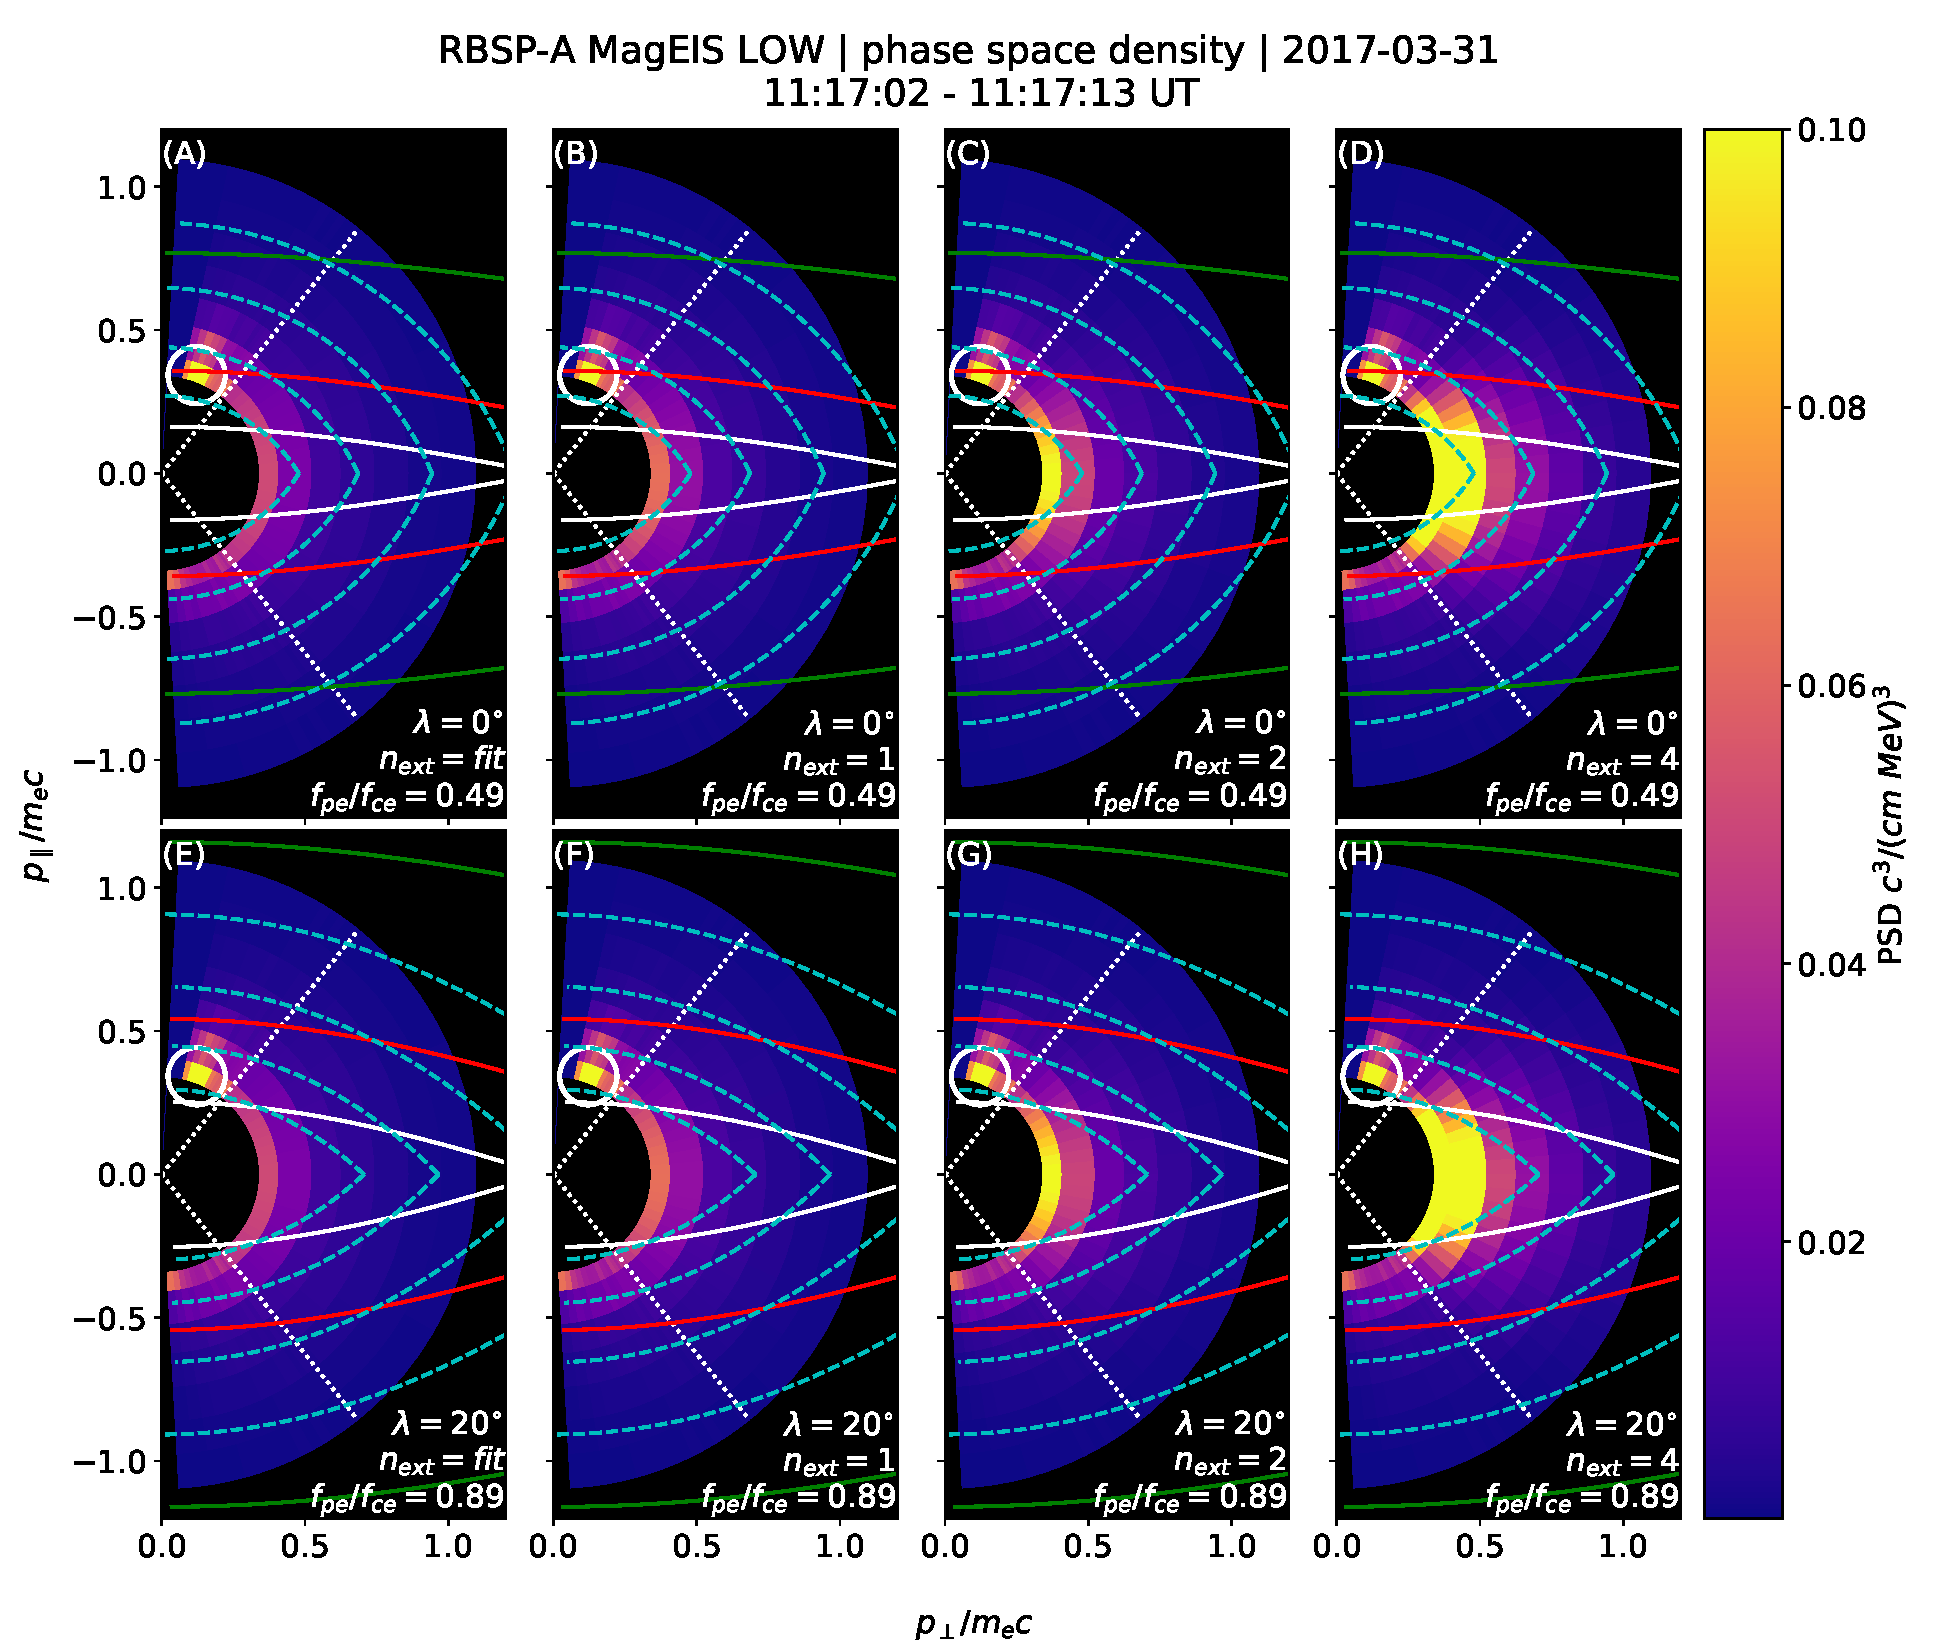
\includegraphics[width=\textwidth]{2_fig3_alpha_neg1_n_1.pdf}
\caption{The colored annulus represents $f(p_\perp, p_{||})$ in normalized momentum space, parallel and perpendicular to the background magnetic field. The microburst $f(p_\perp, p_{||})$ is highlighted with the white circle. The columns show different powers of the sine extrapolation, and rows show the different magnetic latitudes of the scattering. The white dotted traces represent the boundary between the data and extrapolation. The green, red, and white solid traces are the resonance curves for $\omega = 0.2 \Omega_{ce}$, $0.4 \Omega_{ce}$, $0.6 \Omega_{ce}$, respectively. The cyan dashed traces are the diffusion curves for a $\omega = 0.4 \Omega_{ce}$ wave (waves of other frequency have similar diffusion curves). The magnetic latitude of the scattering, the ratio of the plasma to the cyclotron frequency, and the power of the sine extrapolation is annotated in each panel. For the resonance and diffusion curves, the density model assumed a $n_L = 1 \ e^-/cm^3$ and $\psi = -1$.}
\label{fig3}
\end{figure}

\subsection{Motion of resonant electrons in phase space}\label{diffusion_derivation}
To calculate the motion of resonant electrons in momentum space, we used the relativistic theory of wave-particle resonant diffusion developed by \citet{Walker1993} and \citet{Summers1998} and applied in \citet{Meredith2002}. The chorus wave can modify $f(p_\perp, p_{||})$ when a resonance condition is satisfied. The cyclotron resonance condition between an electron with velocity $v = \sqrt{v_{||}^2 + v_{\perp}^2}$ and a parallel propagating wave of frequency $\omega$ and wave number $k_{||}$ is given by
\begin{equation}
\omega - v_{||} k_{||} = \frac{\Omega_{ce}}{\gamma},
\label{res_condition}
\end{equation} where $\Omega_{ce}$ is the electron gyrofrequency at the scattering location, and $\gamma$ is the relativistic correction. Assuming the cold plasma approximation,
\begin{equation}
k_{||} = \frac{\omega}{c} \sqrt{1 - \frac{\omega_{pe}^2}{\omega (\omega - |\Omega_{ce}|)}},
\end{equation} where $\omega_{pe}$ is the plasma frequency. For a particular set of parameters, Eq. \ref{res_condition} defines a curve in momentum space that describes which electrons will resonate with a monochromatic wave.

To calculate $k_{||}$, we approximated the electron number density, $n_e(\lambda)$ locally and at the magnetic equator. Locally, the plasma density was approximately $n_e(\lambda = -20^\circ) = n_L \approx 1 \ cm^{-3}$. We used  magnetospheric seismology techniques \citep[e.g.][]{Takahashi2007} to parameterize $n_e(\lambda)$ elsewhere along the field line with

\begin{equation}
n_e(\lambda) = n_e(0) \bigg( \frac{L R_e}{R(\lambda)} \bigg)^\psi
\label{density_model_basic}
\end{equation} where $R_e$ is the Earth's radius, $R(\lambda)$ is the radial distance from the Earth to the spacecraft, and $\psi$ is the exponent parameter. Assuming a dipole magnetic field for which $R(\lambda) = L R_e \cos^2{\lambda}$ \citep[e.g.][]{Schulz1974}, we can express Eq. \ref{density_model_basic} in terms of $n_L$ via 
\begin{equation}
n_e(\lambda) = n_{L} \bigg( \frac{\cos{\lambda_{L}}}{\cos{\lambda}} \bigg)^{2 \psi}
\end{equation} where we used $\psi = -1$ (higher density at the magnetic equator) in this analysis. We chose this exponent parameter because it is a realistic best case scenario for the electrons to be transported along the diffusion curves (described below).

\citet{Walker1993} and \citet{Summers1998} argued that a resonant electron will move along diffusion curves in momentum space. A diffusion curve is derived as follows. In the reference frame moving with a monochromatic chorus wave's phase velocity (wave frame), the chorus wave is stationary and there is no electric field. Thus in the wave frame, the electron's kinetic energy is conserved, and the electron's velocity in the wave frame can be expressed in differential form as
\begin{equation}
v_{||} dv_{||} + v_{\perp} dv_{\perp} = 0.
\label{ke}
\end{equation} After a Lorentz transformation of Eq. \ref{ke} into the magnetospheric frame, kinetic energy will no longer be conserved. After integration and manipulation of Eq. \ref{ke}, we obtain:
\begin{equation}
\bigg( 1 - \frac{u_0^2 v_0^2}{c^4} \bigg) v_{||}^2 - 2 u_0 \bigg( 1 - \frac{v_0^2}{c^2} \bigg) v_{||} + \bigg( 1 - \frac{u_0^2}{c^2} \bigg) v_\perp^2 = v_0^2 - u_0^2
\label{single_characteristic}
\end{equation} where $u_0 = \omega /k_{||}$ is the phase velocity, and $\mathrm{v}_0$ is a constant of integration \citep{Walker1993, Summers1998}. Equation \ref{single_characteristic} defines a family of diffusion curves in momentum space on which resonant electrons will move. The distance that an electron moves along a diffusion curve is a function of wave and plasma parameters, and is estimated from the magnitude of the diffusion coefficients and the resonance time.

\subsection{Comparing the microburst PSD to diffusion theory} \label{compare_section}
Superposed on the PSD plots in Fig. \ref{fig3} are resonance curves for chorus waves of $\omega = 0.2 \Omega_{ce}$, $0.4 \Omega_{ce}$, $0.6 \Omega_{ce}$ and a few diffusion curves for a $\omega = 0.4 \Omega_{ce}$ wave. These curves were parameterized by $\lambda$ using a dipole magnetic field for $\lambda = 0^\circ$ (Fig. \ref{fig3}, panels A-D) and $\lambda = 20^\circ$ (Fig. \ref{fig3}, panels E-H). If the transport of microburst electrons is consistent with gyro-resonant diffusion, a diffusion curve that passes through the microburst $f(p_\perp, p_{||})$ must also pass through another region with at least the same magnitude PSD ($f(p_\perp, p_{||}) \geq 0.1 \ \mathrm{c^3/(cm \ MeV)^3}$) e.g. Fig. \ref{fig3}, panel (D). With this constraint, an artificially high extrapolated $f(p_\perp, p_{||})$ with $n > 2$ (5 times larger than calculated from the fits) must be assumed for there to have been a sufficient source of PSD anywhere in MagEIS-A's energy range. 

We now show that by comparing MagEIS observations with theory, that the minimum wave amplitude necessary to scatter these electrons is much higher than was observed by EMFISIS-A. If we assume a unrealistic PAD with enough PSD just equatorward of RBSP-A, we can use MagEIS-A observations to calculate the minimum $\Delta \alpha_{eq}$ that the electrons were transported. We then used diffusion theory to calculate the necessary wave amplitude. For microbursts with larger PAs, MagEIS-A observed a transport of $\Delta \alpha_{eq} = 9^\circ$ and for microbursts with smaller PAs, the observed transport was $\Delta \alpha_{eq} = 24^\circ$. The required wave amplitude was calculated with Eq. 3 from \citet{Thorne1980} assuming a maximum resonance period of a quarter bounce. The observed change in PA requires a wave amplitude $0.2 < |B_w| < 0.5$ nT. For a few brief moments, the EMFISIS-A WFR waveform data showed $0.1 < |B_w| < 0.15$ nT, so a transport of $9^\circ$ is plausible, but not likely for $24^\circ$.

Another source of microburst electrons may be from energies below MagEIS-A's range. The Helium, Oxygen, Proton, and Electron mass spectrometer \citep{Funsten2013} on RBSP-A observed $f(p_\perp, p_{||}) \geq 0.1 \ \mathrm{c^3/(cm \ MeV)^3}$ for < 23 keV electrons at this time. We then assumed the wave amplitude derived above to predict the transport in energy. We used the fact that the momentum and pitch angle diffusion coefficients, $D_{pp}$ and $D_{\alpha \alpha}$ are related via $D_{pp}/p^2 \sim D_{\alpha \alpha}$ or equivalently, $\Delta p/p \sim \Delta \alpha$. The observed PA transport corresponds to an energy transport of $6 < \Delta E < 16$ keV. Therefore, this wave can transport $23$ keV electrons from smaller pitch angles to larger pitch angles and would be observed in the $29-41$ keV MagEIS-A channel. However, this wave is insufficient to transport electrons to the $68-92$ keV channel in one interaction. Therefore we conclude that quasi-linear diffusion cannot explain the observed microbursts.

\section{Discussion and Conclusions} \label{discussion} %%%%%%%%%%%%%%%%%%%%%%%%%%%%%%%%%%%%
These novel observations of impulsive electron signatures reported here fall well within the broad definition of a microburst as described in section \ref{Intro}. Their properties were similar to microbursts observed in LEO, with an E-folding energy of $25 < E_0 < 35$ keV \citep{Datta1997, Lee2005, Lee2012}, duration of 150-500 ms \citep{Lorentzen2001a}, observed upper energy limit of 92 keV, and a lack of clear energy dispersion \citep{Breneman2017}. With MagEIS-A's high time and energy resolution, we conclude that these dispersionless microbursts were recently scattered near the spacecraft. Furthermore, RBSPICE-A's PA coverage suggests that these electrons were scattered over a substantial range of PAs, with the highest intensities near $\alpha_L = 90^\circ$. Overall, our observational evidence suggests that on time scales shorter than one bounce period, the chorus wave effectively accelerated trapped electrons over a broad PA range. 

In the theoretical framework of wave-particle resonant diffusion applied to the observed PSD in section \ref{analysis}, we determine that the observed scattering is not consistent with the quasi-linear approximation. The nearest source of sufficient PSD is too far away in phase space to have been transported by the hypothesized quasi-linear process over a timescale shorter than one bounce period (one interaction). A similar conclusion was made by \citet{Mozer2018} who used quasi-linear theory constrained by RBSP wave measurements. They successfully modeled the one second average precipitating flux observed with AeroCube-6 (AC-6) CubeSats during a conjunction, but they were unable to model the AC-6 fluxes on smaller time scales.

To put these microburst observations into a wider magnetospheric perspective, we observed them during the recovery phase of a minimum Dst of -75 nT storm, a statistically favorable time period for microbursts \citep{O'Brien2003}. Furthermore, during the same storm on March 27th, the Arase spacecraft observed highly correlated lower band chorus with 10-50 keV electron precipitation inside the loss cone. At that time, Arase's magnetic field footprint was near The Pas All-Sky Imager (part of the THEMIS mission) which simultaneously observed pulsating auroral patches \citep{Kasahara2018}. While microbursts and pulsating auroral patches have not been clearly connected, they are both believed to be a product of electron scattering by whistler mode waves \citep[e.g.][]{Lorentzen2001a, O'Brien2003, Nishimura2011a, Ozaki2012}.

The combined capabilities of the various RBSP wave and particle instruments enable comprehensive studies of wave-particle scattering and the resulting microburst precipitation. From a preliminary search by the authors, other microburst-like signatures have been found with RBSP. Similar to previous studies \citep[e.g.][]{O'Brien2003, Blum2015}, a statistical study of high-altitude microbursts in L-MLT space needs to be conducted before we can verify that these microbursts are the counterpart of the microbursts observed in LEO and the upper atmosphere.

\section{Acknowledgments}
The authors acknowledge the technicians, engineers, and scientists who made the RBSP and AC-6 missions possible. One author (Shumko) would like to acknowledge Dana Longcope for his help in understanding the quasi-linear diffusion theory. Dr. Gkioulidou was supported by JHU/APL subcontract 131803 to the NJIT under NASA Prime contract NNN06AA01C. EMFISIS work was supported by JHU/APL contract no. 921647 under NASA Prime contract No. NAS5-01072. The MagEIS instrument was funded by NASA's Prime contract no. NAS5-01072. The level 3 MagEIS-A ``high rate" data is available in the Supporting Information, level 1 RBSPICE EBR data is archived at http://rbspicea.ftecs.com/, and the EMFISIS level 2 spectral matrix and burst data as well as the level 3 magnetometer data is archived at http://emfisis.physics.uiowa.edu/data/index. The IRBEM Library can be obtained at irbem.sf.net.